% ===========================================================================
% Appendices C-F: material relocated out of the main body by the short
% variant of this paper. Nothing here is new. Every paragraph, table and
% figure below appears in the full-length build inside the main body, at the
% section named in each subsection heading; the short variant moves it rather
% than dropping it, so that no number, count, disclosure or preregistration
% qualifier is lost. Section cross-references (\S3.4 and the like) point at
% the same sections as in the full build.
% ===========================================================================

\section{Relocated from \S1 and \S2: framing, trap-zone arithmetic, and the recipe family}

\subsection{Source audit of in-loop conditioning (from \S1)}

A source audit finds no cited system making the unconditioned call. FunSearch reseeds emptied
islands by cloning a surviving program, ShinkaEvolve's restart re-seeds from its own archive
(``initial'', ``best'' or ``archive\_random''), and OpenEvolve islands copy the user-provided seed
--- every in-loop call is program-conditioned. The nearest deployed relatives are initializations
conditioned on a seed that ``can be trivial'' (FunSearch) or ``rudimentary'', single-line functions
returning constants (AlphaEvolve), plus AlphaEvolve's ``No evolution'' ablation, which re-prompts
from the same rudimentary program throughout.

For an evolutionary-computation reader the consequence sits at initialization: if generation zero
is one template wearing many coordinates, the diversity machinery downstream --- MAP-Elites
descriptors \citep{mouret2015mapelites}, novelty pressure \citep{lehman2011novelty}, seed
perturbation --- is doing repair rather than exploration. For an evaluation reader it is a floor:
the weak-tier zero-shot mode on this benchmark is computable in advance, so a discovery claim on
circle packing has a known value to beat before any search is credited.

\subsection{Trap zones: branch label versus penalty, the LP gate, and the published-bound coverage gap (from \S1.1)}

\begin{figure}[!ht]
\centering
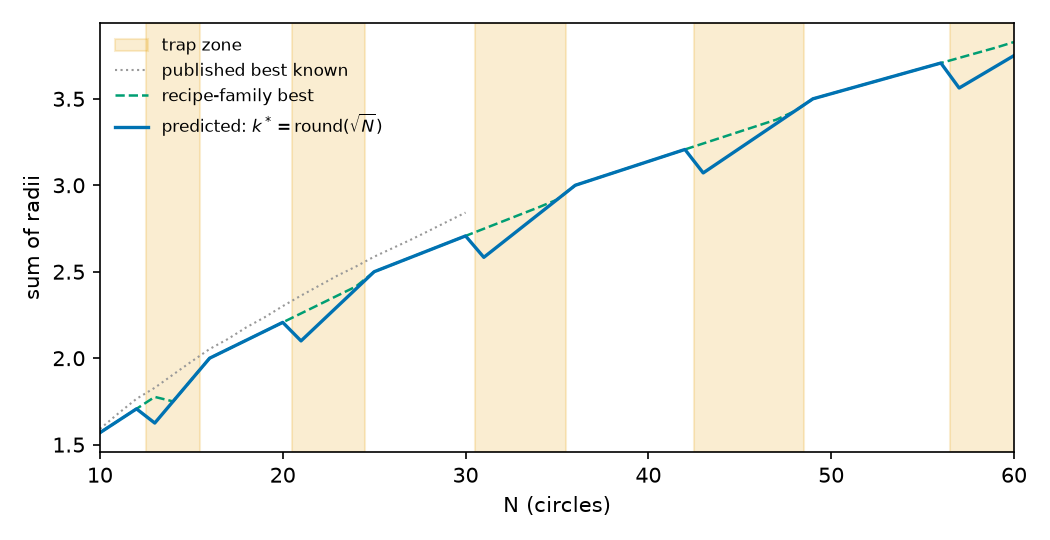
\includegraphics[width=0.78\linewidth]{fig1_trapzones.png}
\caption{\emph{Predicted versus optimal value, $N = 10\ldots60$.} (i) the rule's prediction; (ii) the
best value in the recipe family; (iii, dotted) published best-known values \citep{friedman_packing}, terminating at
$N = 30$ because the bound table stops there. Shaded bands are the trap zones, the last being
$[57,63]$ clipped by \texttt{sweep(10,60)}. Worst-in-zone penalties 8.51\%, 7.03\%, 6.01\%, 5.25\%, 4.66\%; these are
family-internal arithmetic and exact at every $N$, while the published-bound comparison (curve iii)
is checkable only up to $N = 30$, where the bound table stops. The gap
closes to zero at $N = 35$ and $N = 48$ but \textbf{not} at $N = 24$, where 0.59\% remains --- curve (ii)
sits strictly above (i) across $[21,24]$.}
\label{fig:trapzones}
\end{figure}

Branch label and penalty are not coextensive: 4 of the 22 trap-branch $N$ in range cost nothing, so
``trap'' names the branch, not a guaranteed loss. Where the penalty is zero, truncation is
separable from convergence only by structure; \S3.3 uses $N = 35$ as that control.

Every closed-form value is recomputed over the constructed coordinates by an independent linear
program that knows nothing about the recipe; the script aborts on disagreement. 83
configurations, both branches, every $k$ in $2\ldots7$, drift below $10^{-9}$.

Our bound table (\texttt{n\_sweep\_forecast.json}, transcribed from \citet{friedman_packing}) covers $N = 10\ldots30$ only, and its $N = 26$ entry, 2.63598,
\emph{is} ShinkaEvolve's figure truncated, so the LLM-driven systems are the record on this problem. What survives is that the recipe family is never competitive with that
record: deficit 0.02--0.26 across $N = 10\ldots30$, and 0.0946 at $N = 26$
($2.63598 - 2.5414214 = 0.0945586$). Above $N = 30$ there is no bound table, so both the deficit claim and the LP
gate's ``never exceeds a published bound'' abort are unchecked there, covering three of five trap
zones and four of our seven square cells.

\subsection{The recipe family: prior-arm and ledger evidence (from \S2.2)}

The finding that 94 of 95 valid proposals in prior arms were grid-plus-filler is retained only as
motivation, since those arms are not reported here; the self-contained version is the ledger
observation (\texttt{corrections\_ledger.md}, item 30) that across the 155 weak-tier rows collected before arm M only two exceeded the
family best, both by $\sim$$10^{-7}$ --- below the $10^{-6}$ bar, so neither counts as leaving the family under \S5's convention (arm M's 57 rows are scored separately in \S3.4 and were not swept
for this claim).

\subsection{The order rule is a definition, not a fitted law (from \S2.3)}

Given some $k \times k$ grid from this family, ``the nearest
square lattice'' yields $\mathrm{round}(\sqrt{N})$ by construction; $\arg\min_k |k^2 - N|$ switches at
$N = k^2 + k + \tfrac{1}{2}$, $\mathrm{round}(\sqrt{N})$ at $k^2 + k + \tfrac{1}{4}$, so on the integers the two coincide
--- two formalizations of ``nearest'' agreeing signals that no substantive hypothesis
is being selected. Scoring four candidate orders against the three fitting anchors gave
\texttt{nearest} 3/3, \texttt{floor} 2/3, \texttt{argmax} 2/3, \texttt{ceil} 1/3; under a null where each candidate matches
each anchor with probability $\tfrac{1}{2}$, some candidate among four goes 3/3 about 40\% of the time, so
this is a weakly identified discrete selection, not a zero-parameter law.

\section{Relocated from \S3 and \S4: per-arm tables and disclosures}

\subsection{The mode ceiling: structural check and scope conditions (from \S3.2)}

Post-hoc structural check, not preregistered, run after the square arm closed
(\texttt{diagnostics\_kmatch.py}): the grid order backed out of each sample's dominant radius
($k = \mathrm{round}(1/2r)$) equals $k^*(N)$. All 50 of 50 on-prediction samples are $k^*$-structured --- the
value match is not an accounting coincidence --- and 64 of 69 valid samples overall (93\%) sit on
the $k^*$ grid, so most value misses are $k^*$-grid variants (perturbed radii or filler counts), not
different constructions.

Three cells ($N = 17$, 35, 37), all non-discriminating, carry four valid samples each, where a 3/4
mode is thin evidence on its own; the well-populated cells of the held-out probe (\S3.8) are the
stronger test of the same rule. Two scope conditions: this is the bare weak-tier arm --- pooled
over the four discriminating square cells (full ledger), the two higher tiers and the rectangle,
the on-prediction rate is 46\% ($47/102 = 41/57 + 1/30 + 0/4 + 5/11$; the three non-discriminating
square cells, 9/12, are excluded because prediction equals the family argmax there), because \S5's
higher tiers are almost never on-prediction --- and ``modal'' is a property of the observed
sampling regime, not of a pinned decoding configuration (\S8).

\subsection{Forecast versus outcome, and arm F bookkeeping (from \S3.3 and \S4.2)}

\begin{table}[!ht]
\centering
\caption{Forecast versus outcome, both containers.}
\label{tab:forecast}
\small
\begin{tabular}{@{}lcccccc@{}}
\toprule
Cell & Branch & Predicted & Rival argmax & Valid / sampled & On-pred / valid & Rival \\
\midrule
$N{=}13$ (sq) & truncate & 1.6250000 & 1.7761424 & 4/5 $\cdot$ \textbf{18/20} & 3/4 $\cdot$ \textbf{10/18} & 0 \\
$N{=}17$ (sq) & extend & 2.0517767 & $\dagger$ & 4/5 & 3/4 & $\dagger$ \\
$N{=}21$ (sq) & truncate & 2.1000000 & 2.2588835 & 7/10 $\cdot$ \textbf{15/20} & 4/7 $\cdot$ \textbf{12/15} & 2 \\
$N{=}31$ (sq) & truncate & 2.5833333 & 2.7485281 & 5/5 $\cdot$ \textbf{17/20} & 5/5 $\cdot$ \textbf{13/17} & 0 \\
$N{=}35$ (sq) & truncate & 2.9166667 & $\dagger$ & 4/5 & 3/4 & $\dagger$ \\
$N{=}37$ (sq) & extend & 3.0345178 & $\dagger$ & 4/5 & 3/4 & $\dagger$ \\
$N{=}43$ (sq) & truncate & 3.0714286 & 3.2416246 & 7/10 & 6/7 & 0 \\
$N{=}19$, $a{=}3$ & truncate & 3.1666667 & 3.5749194 & 4/8 & 2/4 & 0 \\
$N{=}25$, $a{=}2$ & truncate & 3.1250000 & 3.4832492 & 7/8 & 3/7 & 0 \\
\bottomrule
\end{tabular}

\vspace{0.5ex}
\begin{minipage}{0.95\linewidth}
\footnotesize
Plain entries are the original 45-invocation bare arm (\S3.3's corpus); \textbf{bold} the same cells
over the full 85-row bare ledger after \S6 added 40 rows. $\dagger$ marks non-discriminating cells
(prediction equals family argmax), excluded from rival denominators. Square discriminating
cells: 18/23 and 2/23 on the original corpus; 41/57 and 2/57 on the full ledger. Rectangle:
5/11 and 0/11. Sources: \texttt{arm\_f\_repro.py} over \texttt{arm\_f\_candidates\_v2.jsonl}, \texttt{arm\_g\_rect.py} over
\texttt{arm\_g\_candidates.jsonl}.
\end{minipage}
\end{table}

The original-corpus figures cover the \textbf{original 45-invocation bare arm only} (ids $\le 5$ at
$N = 13/31$, $\le 10$ at $N = 21$, all rows at $N = 17/35/37/43$), the corpus that existed when \S3
was written. \S6 later added 40 bare rows at $N = 13/21/31$ under the same arm label; over the full
shipped ledger the same four cells give 41/57 on-prediction and 2/57 rival. Both are reported.

Five invocations were rejected by the runtime's 20-subagent concurrency cap
\emph{before reaching a model}. We excluded them under a rule that was not preregistered, so the arm
is reported both ways --- $35/45 = 77.8\%$, or $35/50 = 70.0\%$ had the rejections been scored as model
failures --- and the five records appear in the ledger in no form (\S9). The arm
also contains three parse failures, and one $N = 37$ proposer derived
$r = (\sqrt{2}-1)/12$ correctly in prose, then transcribed 0.03571429.

\subsection{Arm M in full (from \S3.4)}

Two gaps remained after the square arm: (i) $V(k, m)$'s filler branch
was empirically supported only at $m \in \{0, 1\}$ --- the converge cells $N = 17$ and 37 both have
$m = 1$ --- and (ii) the $k = 8$ trap zone appeared in Figure 1 but was never sampled. Arm M closes
both gaps and was registered before sampling (\texttt{arm\_m\_preregistration.txt}, commit
\texttt{e528c6b}; prompt hashes in \texttt{arm\_m\_prompts.json}): $n = 15$ bare weak-tier
invocations at each of $N = 20$ ($k^* = 4$, $m = 4$, predicted $V(4,4) = 2.2071068$), $N = 30$
($k^* = 5$, $m = 5$, $V(5,5) = 2.7071068$), $N = 41$ ($k^* = 6$, $m = 5$, $V(6,5) = 3.1725890$) and
$N = 57$ ($k^* = 8$, trap, $T(8,57) = 3.5625000$, rival $V(7,8) = 3.7366935$), with an explicit
tie-stated falsifier for each half.

The registered predictions P-M1--P-M3 are disconfirmed: not one of the three converge cells has
$V(k^*, m)$ as its modal output. The model does not extend a $k^*$-grid with fillers; it moves
\emph{up} to the $(k^*{+}1)$ grid and truncates or exactly fills it --- modal outputs
$2.0 = T(5,20)$ (12 of 15 valid; $N = 20$ is the $5 \times 4$ rectangle exactly), $2.5 = T(6,30)$
(11 of 14; $6 \times 5$ exactly) and $2.9285714 = T(7,41)$ (6 of 7; $7 \times 6$ minus one). Exactly one
sample in 36 valid converge-cell rows emitted the registered construction --- a textbook $V(4,4)$,
all four fillers at $(\sqrt{2}-1)/8$. Per the registered falsifier wording, \textbf{$V(k, m)$ is
restricted to the $m \le 1$ support previously observed}, and the branch rule's extend arm is
disconfirmed at $m \ge 4$; the intermediate ``places some fillers'' outcome named in the
registration did not occur (filler count 0 in 35 of 36 valid converge rows). The emergent
regularity is arithmetic, not geometric: where $N$ factors as $a \times b$ with $a$, $b$ near
$\sqrt{N}$ the model emits that exact rectangle of uniform circles ($20 = 5 \times 4$,
$30 = 6 \times 5$), which is further evidence for \S8's arithmetic-tractability alternative ---
rectangle factorization is mentally computable where filler tangency is not.

Validity by cell: 15/15, 14/15 (one parse failure --- fraction literals), 7/12 and 10/15 at
$10^{-6}$. Three $N = 41$ invocations died in the runtime before reaching a model and are excluded
under the rejection rule registered for this arm in \texttt{arm\_m\_preregistration.txt} ---
registered precisely because the analogous arm F exclusion was not (\S9) --- and counted here: the
cell is $n = 12$ sampled of 15 launched. Raw rows verbatim in \texttt{arm\_m\_collect.jsonl}; scoring
in \texttt{arm\_m\_analysis.py}, conventions identical to arm F.

\textbf{Table M --- Arm M, forecast versus outcome (all four registered cells).}

\begin{center}
\begin{small}
\setlength{\tabcolsep}{3.5pt}
\begin{tabular}{@{}ccp{0.09\linewidth}p{0.16\linewidth}p{0.20\linewidth}ccp{0.16\linewidth}@{}}
\toprule
$N$ & $k^*$ & Branch & Registered prediction & Modal valid output & Freq & Valid / sampled & Verdict \\
\midrule
20 & 4 & extend, $m = 4$ & $V(4,4) = 2.2071068$ & $T(5,20) = 2.0000000$ ($5 \times 4$ exact) & 12/15 & 15/15 & P-M1 \textbf{disconfirmed} \\
30 & 5 & extend, $m = 5$ & $V(5,5) = 2.7071068$ & $T(6,30) = 2.5000000$ ($6 \times 5$ exact) & 11/14 & 14/15 & P-M2 \textbf{disconfirmed} \\
41 & 6 & extend, $m = 5$ & $V(6,5) = 3.1725890$ & $T(7,41) = 2.9285714$ ($7 \times 6 - 1$) & 6/7 & 7/12 & P-M3 \textbf{disconfirmed} \\
57 & 8 & truncate & $T(8,57) = 3.5625000$, rival count 0 & $T(8,57) = 3.5625000$ & 6/10 & 10/15 & P-M4 confirmed; rival 0/10 \\
\bottomrule
\end{tabular}
\end{small}
\end{center}

Exactly one $V(k^*, m)$ construction appears in 36 valid converge-cell rows; filler count is 0
in 35 of 36. Three converge-cell rows leave the recipe family \emph{upward} --- two at $N = 20$ (staggered rows of four at $r = 1/9$, sum 2.2222222, against the family best $V(4,4) = 2.2071068$) and one at $N = 30$ ($r = 1/11$, sum 2.7272727, against $V(5,5) = 2.7071068$; valid at $10^{-6}$, not at $10^{-9}$) --- hexagonal layouts the family does not contain, found by a post-hoc sweep (not preregistered) run after a fourth-round check; they are not the modal output at either cell and do not bear on the discriminating-cell claims. Regenerates from \texttt{arm\_m\_collect.jsonl} via \texttt{arm\_m\_analysis.py}.

\subsection{Arms MU and CH in full (from \S3.5)}

Two questions were still open after arm M. Does the unconditioned anchoring result say anything
about calls that carry a parent program --- the regime evolutionary loops actually run in --- and
does the \S8 arithmetic-tractability alternative survive a direct probe? Arms MU and CH were
registered together before sampling (\texttt{arm\_mu\_preregistration.txt}, commit \texttt{2b7d202};
prompt hashes in \texttt{arm\_mu\_prompts.json}), with numeric decision thresholds, a power analysis
(0.83 at the registered effect size), tie-against conventions, and falsifier F-MU1.

\textbf{Arm MU} issues one-parent mutation calls: the bare prompt plus an existing packing and the
instruction to modify it so the sum of radii increases. Three parents per cell
($N = 13$, 21, 31; $n = 15$ per condition-cell, 135 invocations): \emph{A\_anchor}, the model's own
unconditioned anchor $T(k^*, N)$; \emph{B\_rival}, the provably better in-family rival $V(k^*{-}1, m)$;
and \emph{C\_offfamily}, a diagonal-chain packing scoring $\approx$ 0.59--0.62, far below either.
Every valid B\_rival sample keeps or refines the rival construction, and every one inherits the
rival's grid order. The template does not reassert itself when a better in-family parent is
present. A\_anchor makes the same point from the other side: even with the model's \emph{own} anchor
as parent and an explicit increase-the-sum instruction, only 7 of 28 valid samples (25\%,
CI $[0.13, 0.43]$) stay on the anchor. Per the registered falsifier wording: the unconditioned-call
anchoring result does not transfer to parent-conditioned calls, the loop-relevance framing is
disconfirmed for the one-parent regime, and this paper's claims are scoped to unconditioned calls
throughout. The one condition where the template does reassert itself is the one the registration
predicted it would: given the \emph{off-family} diagonal parent, 20 of 34 valid samples (58.8\%,
CI $[0.42, 0.74]$) abandon the parent entirely and emit a $k^*$-grid construction --- P-MU4 holds
per-cell at $N = 21$ (7/13) and $N = 31$ (12/14, every valid sample on the $k = 6$ grid), though
not at $N = 13$ (1/7). The asymmetry is the finding: a good in-family parent is followed, a bad
off-family parent is discarded for the template. The attractor is real but weak --- it captures
the trajectory only when the parent is worse than what the template supplies.

\textbf{Arm CH} hands the model the entire recipe family: the bare prompt plus every admissible
$T(k, N)$ and $V(k, m)$ value enumerated, including the family argmax, with the instruction to
use whichever scores highest or anything better ($n = 15$ per cell, 45 invocations). The \S8
tractability alternative says the model truncates at $k^*$ because that is the only construction
it can compute; enumerating the family removes the computation burden, so under that reading
the modal output should become the stated argmax (P-CH2). Under the template reading it stays
$T(k^*, N)$ despite the argmax being printed in the prompt (P-CH1). Read no further than the
registered scorer and the tractability alternative fails the probe. But validity is low in this
arm --- 2, 5 and 7 valid of 15 by cell --- and the failure modes reverse the picture at the
\emph{attempt} level: all 31 invalid rows attempt the stated argmax (every one carries the family's
filler radius). Of those, 30 misplace the fillers --- typically at the container corners, where
radius $(\sqrt{2}-1)/(2k)$ overlaps the adjacent grid circle; the correct construction places them
at the grid interstices --- and 1 emits radical literals the registered scorer cannot evaluate.
Counting attempts rather than valid outputs, the model \emph{chooses} the argmax in a large
majority of CH invocations and simply fails to execute it; the valid-conditioned modal is
dominated by the template because the template is the only construction the model executes
reliably. This is the same asymmetry arm MU found from the other direction, and it narrows the
paper's central claim to its defensible core: the template is not what the model prefers; it is
what the model can build.

\textbf{Table MU --- Arm MU, registered thresholds versus outcome, by parent condition (pooled
over $N = 13$, 21, 31).}

\begin{center}
\begin{small}
\setlength{\tabcolsep}{3.5pt}
\begin{tabular}{@{}p{0.15\linewidth}cp{0.13\linewidth}p{0.13\linewidth}p{0.10\linewidth}p{0.08\linewidth}p{0.24\linewidth}@{}}
\toprule
Parent & Valid & Anchor-rate (CI) & Registered threshold & Keep-or-improve & $k$-inher. & Reading \\
\midrule
\emph{B\_rival} (in-family argmax) & 26 & 0/26 (0\%, $[0.00, 0.13]$) & DISSOLVES if $\le$ 20\% & 26/26 (bar $\ge$ 50\%) & 26/26 & \textbf{F-MU1 triggered} --- anchoring does not transfer to one-parent calls \\
\emph{A\_anchor} (model's own anchor) & 28 & 7/28 (25\%, $[0.13, 0.43]$) & P-MU1 predicted $\ge$ 50\% & --- & --- & not met --- even the anchor-as-parent does not hold the anchor \\
\emph{C\_offfamily} (diagonal, $\approx$0.6) & 34 & 20/34 abandon parent for $k^*$-grid (58.8\%, $[0.42, 0.74]$) & P-MU4: template reasserts & --- & --- & holds at $N = 21$, 31; not at $N = 13$ (1/7) \\
\bottomrule
\end{tabular}
\end{small}
\end{center}

\textbf{Table CH --- Arm CH, valid-conditioned verdict versus attempt-level decomposition.}

\begin{center}
\begin{small}
\setlength{\tabcolsep}{3.5pt}
\begin{tabular}{@{}ccp{0.24\linewidth}cp{0.22\linewidth}p{0.21\linewidth}@{}}
\toprule
$N$ & Stated argmax & Modal valid output & Valid & Invalid rows attempting argmax & Registered verdict \\
\midrule
13 & 1.7761424 & $T(4,13) = 1.6250000$ & 2/15 & all & P-CH1 holds \\
21 & 2.2588835 & argmax, 3/5 & 5/15 & all & P-CH2 (argmax) \\
31 & 2.7485281 & $T(6,31) \approx 2.5833$ (4/7) & 7/15 & all & P-CH1 holds (one-sample margin) \\
pooled & --- & template 2 of 3 cells & 14/45 & \textbf{31/31} (30 misplaced fillers, 1 unevaluable radicals) & choice follows score table; execution fails off-template \\
\bottomrule
\end{tabular}
\end{small}
\end{center}

Raw rows verbatim in \texttt{arm\_mu\_collect.jsonl} (180 of 180 launched invocations collected across arms MU and CH, no
runtime deaths); scoring in \texttt{arm\_mu\_analysis.py}, committed before sampling completed; frozen
output in \texttt{arm\_mu\_results.txt}. This arm brings the study corpus to 468 invocations.

\subsection{Arms GM3 and V in full (from \S3.6)}

\textbf{Table CV --- Cross-vendor verdicts, both instruments.}

\begin{center}
\begin{small}
\setlength{\tabcolsep}{3.5pt}
\begin{tabular}{@{}p{0.10\linewidth}p{0.13\linewidth}p{0.14\linewidth}p{0.20\linewidth}p{0.32\linewidth}@{}}
\toprule
Vendor & Model & Instrument & Registered test & Verdict \\
\midrule
Google & gemma-4-26b & first-party API, 7 $N$ $\times$ 20 (41/140 rows routed under amendment; dual accounting) & pooled $\ge$ 30\%; cell-level $\ge$ 5; falsifier $\ge$ 4 fails & pooled bar met (57.5\%); discriminating cells 11/43 = 26\%, \textbf{below} the bar; cell-level short (2/5, falsifier not triggered); all three misses are the \emph{rival construction} (27/43) \\
Cohere & north-mini-code & free-tier alias, 5 $N$ $\times$ 5 & V1 $\ge$ 50\% of valid on-prediction; V2 rival $\le$ 10\% & \textbf{TRANSFERS}, point-estimate (8/12 = 67\%; CI includes bar); V2 HOLDS (0/4) \\
OpenAI (open-weight) & gpt-oss-20b & free-tier alias, 5 $N$ $\times$ 5 & same & \textbf{TRANSFERS}, point-estimate (11/18 = 61\%; CI includes bar); V2 HOLDS (0/9) \\
Google & gemma-4-31b & free-tier alias, 5 $N$ $\times$ 5 & same & \textbf{DOES-NOT-TRANSFER} (0/15); V2 HOLDS (0/3) \\
10 further aliases & (NVIDIA, Liquid, Poolside, inclusionAI, others; one unattributed) & free-tier & floor: $\ge$ 10 of 25 invocations valid & BELOW-FLOOR; failure taxonomies logged, no claim in either direction \\
\bottomrule
\end{tabular}
\end{small}
\end{center}

\textbf{Arm GM3.} Arm GM3 asks whether the anchoring law is a
fact about the original lineage or about weak-tier models as a class, by re-running the
unconditioned-call protocol against a second vendor's open-weight family
(gemma-4-26b-a4b-it) through its first-party API: seven $N$ cells, twenty samples each,
registered predictions and falsifier fixed before sampling (prereg chain in \S9; the
instrument's history --- a first attempt whose 4,096-token budget was consumed entirely by the
model's deliberation channel, resolved by a registered re-run at 16,384 --- is in \S8 and
Appendix~F.1, and is itself a finding about output-budget confounds in cross-vendor comparisons).
Per cell, recomputable from \texttt{arm\_gm\_gm3\_checkpoint.jsonl} by \texttt{arm\_gm3\_analysis.py}
with no arguments:

\begin{center}
\begin{tabular}{@{}ccccccc@{}}
\toprule
$N$ & predicted (4 dp) & Gemma modal sum & mode freq & valid $n$ & on-prediction & MODE-MATCH \\
\midrule
13 & 1.6250 & 1.7761 & 7/9 & 9 & 0 & no (misses upward) \\
17 & 2.0518 & \textbf{2.0518} & 19/20 & 20 & 20 & \textbf{yes} \\
21 & 2.1000 & 2.2589 & 9/18 & 18 & 8 & no (misses upward) \\
31 & 2.5833 & 2.7485 & 11/16 & 16 & 3 & no (misses upward) \\
35 & 2.9167 & \textbf{2.9167} & 15/15 & 15 & 15 & \textbf{yes} \\
37 & 3.0345 & --- & --- & 2 & 0 & UNSCOREABLE \\
43 & 3.0714 & --- & --- & 0 & 0 & UNSCOREABLE \\
\bottomrule
\end{tabular}
\end{center}

\begin{figure}[!ht]
\centering

\includegraphics[width=\linewidth]{fig_gm3_anchoring.png}
\caption{\emph{Arm GM3 modal sums against the registered prediction.} Filled green circles match the
predicted mode (the dashed line is $V(k^*, m)$ at extend cells and $T(k^*, N)$ at truncate cells) (frequencies annotated); open red triangles miss --- every miss lands above the
prediction, on the rival argmax (the modal packings carry the rival's two-radius structure,
27/27 --- \S3.6); the two largest cells are UNSCOREABLE under the registered $<$3-valid rule.
Regenerates via \texttt{fig\_gm3\_anchoring.py} from \texttt{arm\_gm3\_report.json} (itself replayed from the
raw ledger by \texttt{arm\_gm3\_analysis.py}, no arguments).}
\label{fig:gm3anchoring}
\end{figure}

The registered metric pools all cells, and the pass rides on that: by \S3.2's own convention ---
arm F's pooled rate excludes non-discriminating cells \emph{because prediction equals the family
argmax there} --- the decomposition must be stated. 35 of the 46 on-prediction packings sit in the
two non-discriminating cells (20/20 at $N = 17$, 15/15 at $N = 35$); on the three discriminating
cells the rate is 11 of 43 (25.6\%), below the bar the pooled metric passes. \textbf{The structural
signature came in under its bar}: 20 of 46 on-prediction samples (43\%, bar: half) carry the exact
two-radius grid-plus-filler decomposition. The instrument is blind by construction at truncate
cells, whose prediction is single-radius: all 20 signatures come from $N = 17$ (20 of 20), the one
extend cell among the matches, while $N = 35$'s 15 on-prediction truncations carry no filler to
detect (0 of 15). The registered verdict stands as registered; read per eligible cell, the
construction matches wherever it can be seen.

The registered signature instrument could not see the rival structure on the miss side: it tests
radii against the \emph{predicted} order $k^*$, so it is structurally blind to $(k^*{-}1)$
constructions --- which is why the 43\% signature figure coexists with a 100\% rival-structure rate
on the miss side. Read against \S8's tractability alternative, the anchor value marks where
construction-by-mental-arithmetic lands, and a family with more arithmetic reach executes the
harder in-family construction rather than truncating --- same recipe family, other branch.

\textbf{Arm V.} Arm GM3 varied the vendor while holding the instrument close to laboratory grade ---
first-party API, pinned temperature, explicit output budget, seven cells at twenty samples.
Arm V varies vendor and serving class at once, under the same byte-identical arm-F prompts
both arms inherit (SHA-256 per $N$ restated in the registration and recomputed at call time,
aborting on mismatch; the GM-chain registration pins the identical hashes), at five cells and
five samples per (model, $N$), against free-tier aliases
across seven attributed vendors (\texttt{arm\_v\_preregistration.md}, committed before sampling; three amendments,
each committed before the sampling it governs, expanded the original three-alias design to
thirteen aliases across two serving paths --- the opencode CLI and OpenRouter chat-completions ---
and raised \texttt{max\_tokens} to 24,576 after hidden-reasoning truncation emptied three models'
replies). Serving disclosures per the companion paper's protocol: aliases on managed paths,
\texttt{sampling\_params: null} on every row, per-row upstream-provider strings logged where the path
reports them, every invocation appended live to \texttt{arm\_v\_candidates\_raw.jsonl} --- 877
invocations, failures and refusals included. Scoring is \texttt{arm\_f\_repro.py}'s
parse/validate/classify unchanged, tolerances registered in arm F before its sampling.

Registered floor: $\ge$10 of a model's 25 registered invocations valid at $10^{-6}$; below it, no
anchoring claim in either direction. Execution retried each invocation slot until content
arrived, per amendment 3's registered transport-repair and accounting rule, so the ledger
holds many more attempt rows than slots --- gemma-4-31b's 25 slots, for instance, took 190
attempt rows, 165 of them transport failures --- and the floor is evaluated on the 25 slots,
not the attempts. Ten of thirteen aliases finished BELOW-FLOOR --- including all three
originally-registered opencode aliases, whose logged failure taxonomies are
transport-dominated for one (CLI build banners, timeouts, ``Unknown model'' errors as the
free tier rotated its catalogue) and roughly half transport, half parse-failure for the
other two --- plus one alias returning all 108 of its attempts without content. Three aliases
cleared the floor, and their registered verdicts split:

\begin{center}
\footnotesize
\setlength{\tabcolsep}{3.5pt}
\begin{tabular}{@{}lcccc@{}}
\toprule
alias (vendor) & valid & V1 on-prediction & V1 verdict (bar: $\ge$50\%) & V2 rival-argmax (bar: $\le$10\%) \\
\midrule
\texttt{north-mini-code} (Cohere) & 12 & 8/12 [39--86\%] & \textbf{TRANSFERS} (point est.) & 0/4 $\rightarrow$ \textbf{HOLDS} \\
\texttt{gpt-oss-20b} (OpenAI, open-weight) & 18 & 11/18 [39--80\%] & \textbf{TRANSFERS} (point est.) & 0/9 $\rightarrow$ \textbf{HOLDS} \\
\texttt{gemma-4-31b-it} (Google) & 15 & 0/15 = 0\% & \textbf{DOES-NOT-TRANSFER} & 0/3 $\rightarrow$ \textbf{HOLDS} \\
\bottomrule
\end{tabular}
\end{center}

The registration (\texttt{arm\_v\_preregistration.md}) recorded the original family's prior for the
strong-form statistic as 0/21 over $N \in \{13, 31\}$ only --- a narrower scope than \S3.3's 2/23,
whose two rival hits both sit at $N = 21$, so the two corpora agree at 0 on the registration's own
cells; \S3.6's gemma-4-26b, under the GM-chain instrument, is the standing exception --- its
discriminating-cell mode \emph{is} the rival. And the transfer is not universal: gemma-4-31b,
clearing the same floor, lands the prediction never. Its valid packings are unanchored and low
(bests 0.88--1.85 against predictions 1.63--3.03) --- not the rival, not the template, just weaker
de-novo construction.

The gemma pair needs stating precisely, because this family now appears on both sides, and
the prompts are identical across the two arms --- what differs is parameter count, serving
path and sample budget, not the elicitation. Under the GM-chain instrument (first-party,
pinned temperature, $7 \times 20$), gemma-4-\textbf{26b} met the pooled bar at 57.5\% while its discriminating-cell rate (26\%) fell below it (the mixed-serving
accounting; first-party-only, 59.0\% --- \S8's registered deviation applies to this figure)
while emitting the \emph{rival} construction at 63\% of discriminating-cell validities; under arm
V's free-tier instrument ($5 \times 5$), gemma-4-\textbf{31b} through a rate-starved alias (Google AI
Studio upstream; 27--38 of each cell's attempts returned as shared-pool 429s before content
arrived) lands neither the prediction nor the rival --- its valid packings are weaker de-novo
constructions. The pair bounds the family's behaviour rather than contradicting itself ---
one member sits \emph{above} the template's execution reach (far enough to build the
drop-and-fill rival the original family cannot), the other lands below it --- but model
variant and instrument quality change together across the two measurements, so which
difference carries the split is not attributable from this pair; either way, no
single-model measurement would have seen the boundary.

\subsection{Arm CC in full (from \S3.7)}

The design was registered and pushed to the public remote before sampling
(\texttt{arm\_cc\_preregistration.txt}, commit \texttt{285deca}): the three trap cells
$N = 13, 21, 31$, $n = 15$ weak-tier invocations per cell, prompt equal to the bare stem with
exactly two registered line replacements --- the code-free clause becomes a program contract
(standard-library \texttt{math} only, stated in the prompt) and the output clause asks for program
source. Programs run sandboxed (\texttt{python -I}, 10-second timeout, registered AST allowlist;
the executor and its four-bin smoke test were committed with the registration), and stdout is
scored by arm-F conventions unchanged.

\begin{center}
\begin{small}
\setlength{\tabcolsep}{4pt}
\begin{tabular}{@{}ccccc@{}}
\toprule
$N$ & Valid & Modal bucket (count, margin) & Anchor-rate & Above anchor \\
\midrule
13 & 12/15 & anchor 1.6250000 (2/12, one sample) & 2/12 & 2 --- 1.6614054, and the family argmax exactly \\
21 & 13/15 & anchor 2.1000000 (9/13, margin 8) & 9/13 & 0 \\
31 & 12/15 & anchor 2.5833333 (3/12, one sample) & 3/12 & 0 \\
\bottomrule
\end{tabular}
\end{small}
\end{center}

The registered decomposition row sharpens arm CH rather than repeating it: handed the family's
values, the model chooses the argmax and cannot build it by direct emission (30 of 31 invalid,
\S3.5); allowed to delegate the arithmetic to an executed program, it reaches the same argmax once
in 37 valid outputs and never passes it. Failure taxonomy: 7 of 45 programs produce geometrically
invalid packings, 1 imports \texttt{random} against the stated contract (caught by the registered
gate), none time out. Structural $k = k^*$ in 18 of 37 valid outputs. The lost mass is greedy
radius-growth heuristics converging under the lattice.

Scope, registered before sampling: this instrument measures externally-executed
standard-library arithmetic, not library-assisted optimization --- deployed loops permit
\texttt{numpy}/\texttt{scipy}, and the antecedent study's unconstrained agents wrote
\texttt{scipy} optimizers unprompted, which is why the constraint is stated in the prompt
rather than silently enforced; the library channel remains a further arm. Under the
registration's framing map the P-CC1 branch reads: anchoring extends into the math-only code
channel at these cells, and \S2.1's ``a code channel routes around the anchor'' is weakened
from an assumption to a measured negative --- the routing exists, and for this proposer it does
not lead out of the family. Raw rows verbatim in \texttt{arm\_cc\_collect.jsonl} (45 of 45
launched invocations collected, no runtime deaths); scoring \texttt{arm\_cc\_analysis.py};
frozen report \texttt{arm\_cc\_report.json} and summary \texttt{arm\_cc\_results.txt}.

The Sonnet-tier programs of arm CCS are qualitatively different search --- simulated annealing over
hand-rolled linear-congruential generators, Halton-sequence multi-restarts, force-directed
relaxation, against the weak tier's greedy radius growth --- yet their executed math-only search
never passes the family ceiling at any cell.

Taxonomy for the follow-ups: CC2 41 valid, 3 geometry-invalid, 1 blocked import; CCS 37 valid, 7
geometry-invalid, 1 timeout (the programme's first). One protocol note, disclosed: a single CC2
invocation ($N = 13$, slot 2) used runtime tools despite the no-tools dispatch wrapper; per the
arm-M convention its verbatim final message is scored like every other row. Ledgers
\texttt{arm\_cc2\_collect.jsonl} and \texttt{arm\_ccs\_collect.jsonl} (45/45 each, no runtime deaths);
runner \texttt{arm\_cc2\_analysis.py} reuses CC's registered pipeline unmodified. These arms bring
the study corpus to 603 invocations.

\subsection{Arm CN in full (from \S3.8)}

The $m \ge 4$ branch is already disconfirmed by arm M and was not re-tested. Cells with fewer than
five valid outputs were to be reported UNDERPOWERED; ties for the mode count against the
prediction.

\begin{center}
\begin{footnotesize}
\setlength{\tabcolsep}{4pt}
\begin{tabular}{llllllll}
\toprule
$N$ & $k^*$, prediction & disc. & valid [Wilson 95\%] & on-pred. & mode (count, margin) & verdict & $k^*$-struct. \\
\midrule
50 & 7, $V(7,1) = 3.5295867$ & no & 11/15 [48--89\%] & 4 & 3.5122554 (6, $+2$) & \textbf{MISS} & 10/11 \\
58 & 8, $T(8,58) = 3.6250000$ & yes & 14/15 [70--99\%] & 12 & 3.6250000 (12, $+11$) & \textbf{HIT} & 14/14 \\
62 & 8, $T(8,62) = 3.8750000$ & yes & 13/15 [62--96\%] & 13 & 3.8750000 (13, $+13$) & \textbf{HIT} & 13/13 \\
65 & 8, $V(8,1) = 4.0258883$ & no & 13/15 [62--96\%] & 9 & 4.0258871 (9, $+7$) & \textbf{HIT} & 12/13 \\
75 & 9, $T(9,75) = 4.1666667$ & yes & 12/15 [55--93\%] & 8 & 4.1666667 (8, $+6$) & \textbf{HIT} & 8/12 \\
\bottomrule
\end{tabular}
\end{footnotesize}
\end{center}

At the largest cell, $N = 75$, the four off-mode outputs are alternative constructions (a
$5 \times 15$ grid, twice; a hexagonal layout; a 12-column layout), none of them the rival
$V(8,11)$. The invalid rows are nine overlaps, two count errors and one output of fraction literals
the registered parser does not evaluate (the CH ``radical literal'' mode). Raw rows in
\texttt{arm\_cn\_collect.jsonl} (75/75 launched, none lost); eleven $N = 65$ rows were
transcribed by reconstructing the standard $8 \times 8$ grid string from the emitted filler
triple, flagged per row (\texttt{reconstructed: true}) and disclosed in \texttt{arm\_cn\_results.txt}; the reconstruction is character-identical for these standard grids, but a reader who discards those rows leaves $N = 65$ with three valid samples, below the five-row floor, and P-CN1 at 3 hits of 4 evaluable cells --- the three discriminating cells, which carry the contamination argument, are untouched. The arm brings the study corpus to 678
invocations.

\subsection{Rectangle transfer: all eleven valid proposals (from \S4.1)}

We characterize all eleven here. On-prediction: two
at $N = 19$/$a = 3$ (3.1666666667 and 3.16666673, the latter agreeing to six decimals not seven) and
three at $N = 25$/$a = 2$ (3.125 exactly). Off-prediction at $N = 25$/$a = 2$: two samples emitted a
uniform $5 \times 5$ grid at $r = 0.1$ summing to 2.5000000 --- the \emph{square} rule with no aspect correction,
$k = \mathrm{round}(\sqrt{25}) = 5$ --- plus one at 3.0 and one at 3.151875, the latter above the 3.125 prediction from outside the family and below the rival. At $N = 19$/$a = 3$, \textbf{two} further samples
exceeded the prediction from outside the family, 3.45 and 3.5, both below the rival.

\section{Relocated from \S5 and \S6: tier-ladder and elicitation detail}

\subsection{Three attractor families at one cell (from \S5)}

\begin{figure}[!ht]
\centering
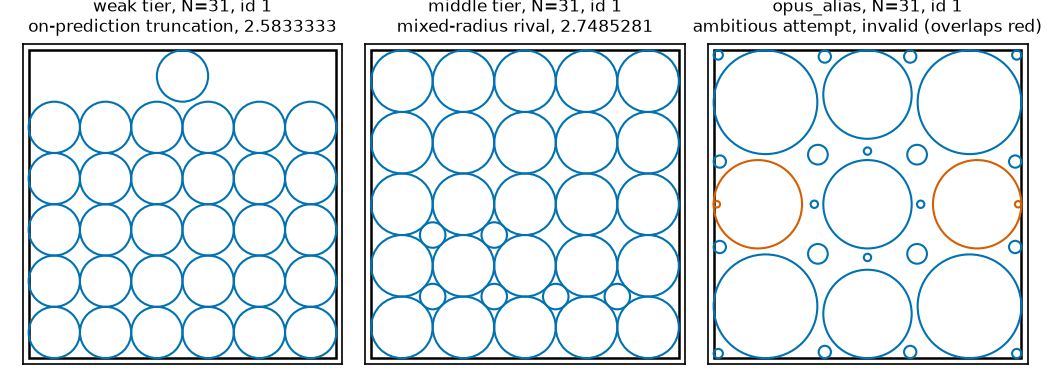
\includegraphics[width=\linewidth]{fig2_packings.png}
\caption{\emph{Three attractor families at a single cell, $N = 31$.} One representative packing
per tier, ledger sample id in each panel title (weak tier \texttt{bare} id 1, on-prediction truncation
2.5833333; middle tier \texttt{sonnet\_bare} id 1, mixed-radius rival 2.7485281; \texttt{opus\_alias} id 1,
invalid, with only the offending circles highlighted). Source: \texttt{arm\_f\_candidates\_v2.jsonl} via
\texttt{fig\_scripts.py}, deterministic (the exemplar rows' geometry is byte-identical in v1; v2 differs
only in provenance metadata).}
\label{fig:packings}
\end{figure}

\subsection{The $N = 31$ scoring defect in full (from \S5)}

One Sonnet sample at $N = 31$ emitted 27 circles at $r = 1/12$ with 4 corner circles at $r = 1/8$,
summing to 2.7499999991 --- above 2.7485281, the best the family reaches at that $N$. Recomputed
from its stored coordinates, the construction is tangency-tight: minimum pairwise and wall slack
both exactly zero at tolerance zero, the exactly-tangent contacts involving the binary-exact
$r = 1/8$ corner circles while the $r = 1/12$ circles carry small positive slack. It is the only
sample in the swept corpus (the 155 weak-tier rows before arm M, \S2.2, plus the higher tiers) to leave the recipe family upward; arm M's converge cells, scored separately, hold three more (\S3.4).

That sample also exposes a scoring defect. At $N = 31$ the family rival (2.7485281) and this
out-of-family value (2.75) differ by $1.47\times10^{-3}$, \emph{inside} the registered $2\times10^{-3}$ window, so the
value classifier counted the escape as a hit on the construction it exceeded. The window was
chosen for the anchor comparison, where the nearest competing value is $\sim$0.15 away, and reused
where it does not fit. Classified by structure instead, Sonnet's rival count at $N = 31$ is 2/10
and pooled 5/30. Every categorical claim in this paper about ``reached the
rival'' or ``left the family'' is made at structure level or at $10^{-6}$, never at $2\times10^{-3}$.

\subsection{The \texttt{opus\_alias} tolerance diagnostic (from \S5)}

Failures are geometric rather than numerical --- edge strips at $r = 0.03$ placed 0.138 from an
$r = 1/6$ grid circle needing 0.197 --- and twice the arm padded to count with zero-radius circles.
A post-hoc diagnostic (not preregistered; labeled as such in the repository) finds no tolerance
artifact behind the 13\%: 24 of 26 invalid samples overlap grossly (median maximum overlap
$3.3\times10^{-2}$; radius-shrink repair costs a median 15\% of sum-of-radii), while tolerance-scale
near-misses ($< 2.5\times10^{-5}$) fall instead in 5 of 7 geometry-scored weak-tier failures --- the
exact-tangency grids, not the ambitious constructions.

\subsection{The ambition diagnostic (from \S5)}

A post-hoc diagnostic (disclosed; \texttt{diagnostics\_ambition.py}, all samples with emitted
geometry, invalid included) gives median distinct radii per sample 1 $\rightarrow$ 2 $\rightarrow$ 3
(means 1.33 $\rightarrow$ 2.40 $\rightarrow$ 3.37) and median off-lattice center fraction 0.08
$\rightarrow$ 0.43 $\rightarrow$ 0.95 across the three tiers --- monotone on both operationalizations.

\subsection{Running corpus arithmetic (from \S6.1)}

The scaled arm ran 100 new invocations, bringing both arms to 20 per cell at
$N \in \{13, 21, 31\}$ and the corpus to 215 logged square invocations (85 bare = 45 original + 40
new; 70 trace = 10 pilot + 60 trace\_v2; 30 sonnet; 30 \texttt{opus\_alias}), plus 16 rectangle
invocations, 231 total before the extension arms. The 20 pre-existing bare rows named in \S6.1 are
$N = 13$ ids 1--5, $N = 21$ ids 1--10 and $N = 31$ ids 1--5.

Arm M (\S3.4) added 57 sampled weak-tier invocations (60 launched), bringing the study corpus to
288; arms MU and CH (\S3.5) added 180 more (180 launched, none lost); the code-channel arms CC, CC2
and CCS (\S3.7) added 135 more (135 launched, none lost), bringing the unconditioned-and-elicitation
corpus to 603; and the held-out-$N$ probe CN (\S3.8) 75 more, to 678. The cross-vendor chain is
scored under its own registrations and adds 420 GM-chain invocations (\S3.6, \S8) and 877 arm-V
attempt rows over 325 registered invocation slots (\S3.6).

\subsection{The paired trace grid (from \S6.2)}

\begin{table}[!ht]
\centering
\caption{Paired trace grid (scaled arm only).}
\label{tab:tracegrid}
\begin{tabular}{@{}llcccc@{}}
\toprule
$N$ & Arm & $n$ & Valid (parse / geom. fail) & On-pred / valid & Rival \\
\midrule
13 & bare & 20 & 18 (0 / 2) & 10 (56\%) & 0 \\
13 & trace\_v2 & 20 & 18 (0 / 2) & 16 (89\%) & 0 \\
21 & bare & 20 & 15 (1 / 4) & 12 (80\%) & 2 \\
21 & trace\_v2 & 20 & 18 (0 / 2) & 16 (89\%) & 0 \\
31 & bare & 20 & 17 (2 / 1) & 13 (76\%) & 0 \\
31 & trace\_v2 & 20 & 17 (0 / 3) & 14 (82\%) & 1 \\
\textbf{pooled} & bare & 60 & 50 (3 / 7) & 35 (70\%) & 2 \\
\textbf{pooled} & trace\_v2 & 60 & 53 (0 / 7) & 46 (87\%) & 1 \\
\bottomrule
\end{tabular}
\end{table}

\begin{figure}[!ht]
\centering
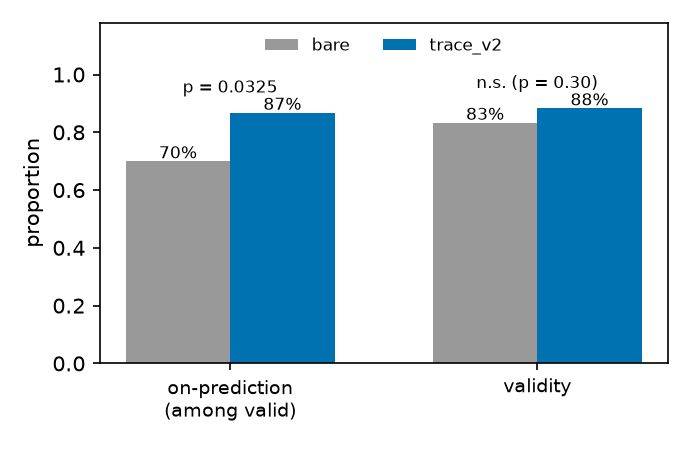
\includegraphics[width=\linewidth]{fig3_armT.png}
\caption{\emph{Bare versus \texttt{trace\_v2}, pooled over cells.} The annotated $p = 0.0325$ is uncorrected and fails the Holm threshold (\S6.4); per-cell values are in the text. Caption caveat: the bars pool the
bare arm's two collection waves, which \S6.4 shows drift materially, so the pooled bare bar is a
mixture; the same-wave comparison in \S6.4 is the wave-controlled picture.}
\label{fig:armT}
\end{figure}

\subsection{Limits of P-T3, in full (from \S6.4)}

\emph{No registered alpha.} P-T3 registered direction only; the $p$-value is a post-hoc addition.

\emph{Multiplicity.} Of four registered predictions, three are reported with $p$-values. Holm sets the
first threshold at $0.05/3 = 0.0167$; $p = 0.0325$ fails it, as it fails Bonferroni at any $m \ge 2$ and
Benjamini--Hochberg FDR at $q = 0.05$. Two-sided Fisher is $p = 0.0537$. P-T3 is nominally significant
uncorrected and is not under family-wise error control.

\emph{Concentration in one cell.} Per-cell tests give $p = 0.030$, 0.41, 0.50
(Table~\ref{tab:tracegrid}); the pooled 17-point gap is a 33-point gap at $N = 13$ averaged with 9-
and 6-point gaps elsewhere, driven by a \emph{low bare rate at $N = 13$} ($10/18 = 56\%$) rather than
a high trace rate --- the trace rate there (89\%) equals that at $N = 21$. Dropping $N = 13$, the
comparison is 30/35 vs 25/32, $p = 0.31$.

\emph{Wave confound.} The bare arm mixes two collection waves; trace\_v2 is one. Splitting bare on the
registered id boundary, with no intervention applied to either half, on-prediction is: $N = 13$, 3/4
old wave vs 7/14 new; $N = 21$, 4/7 vs 8/8; $N = 31$, 5/5 vs 8/12 --- the control arm's own
between-wave drift is comparable to the effect attributed to the manipulation. (An earlier
draft printed 2/4 vs 10/11 at $N = 21$ and a 25/37 pooled figure --- arithmetically impossible
against \S6.1's id boundary; corrected here from the ledger.) Restricting to one
wave, new-wave bare is 23/34 (68\%) against trace\_v2's 46/53 (87\%), but \textbf{this stratified
comparison is post hoc, not preregistered, no confirmatory weight} --- a diagnosis, not a rescue:
wave is a confound \emph{in the registered analysis}, which cannot separate it from the manipulation.
The design fix, interleaved collection in one session, was not run.

\subsection{The twelve exclusions of the registered faithfulness scorer (from \S6.5)}

Nine of the registered scorer's 12 exclusions are regex
coverage gaps, not claims without numeric content: \texttt{DIMS\_RE} matched only the
literal \texttt{NxN} form and \texttt{ROWSCOLS\_RE} required rows before columns, so these fell through despite
carrying explicit checkable dimensions --- ``Regular 3 by 4 grid with one additional circle in row
4''; ``3 complete rows of 4 circles and 1 centered circle in the top row''; ``rectangular grid 4-4-4-1
with uniform radius 1/8''; ``Four-row grid with 4 circles in the first row and 3 in each of the
remaining''; ``Rectangular grid arrangement with 5 columns and 4 rows, plus one additional circle on
top edge''; ``Square grid 5 columns 4 rows with 1 additional circle at top''; ``Rectangular grid six
columns by six rows radius one-twelfth with five circles removed''; ``Regular 5-column by 6-row grid
plus one additional circle in the right margin''; ``Rectangular grid packing with five columns and
six rows plus one additional circle''. Three further exclusions --- ``Uniform horizontal strips with
tight row spacing'', ``Regular rectangular grid packing with corner circle'', ``Equal-radius
rectangular grid with 4 rows stacked vertically'' --- are closer to genuinely unscoreable.

\subsection{Design and bundling disclosure, exact diffs (from \S6.1)}

The pilot's trace prompt had drifted from the bare template beyond the method line --- it omitted
the \texttt{[0,1]x[0,1]} tokens and reworded the output-format line --- so the pilot's intervention
was method-line-plus-rewording, bundled.

The scaled prompt, \texttt{trace\_v2}, is itself a \textbf{bundled prompt-format-and-trace-request}
intervention, though a near-minimal diff: one inserted \texttt{METHOD:} line, plus \texttt{"After
the METHOD line, "} prepended to the output line and \texttt{"no other text"} changed to
\texttt{"no other text after the list"}. That second change is not cosmetic --- \S6.2 shows it
doing measurable work --- so the measured effect is
\emph{method-line-plus-output-line-rewording}, not the method line alone: a weaker version of the
confound for which the pilot was discarded, held to the same standard. The Fisher exact test comes
from the hypergeometric tail in \texttt{arm\_t\_analysis.py}, checked against a reference.

\subsection{The registered falsifier, both readings, in full (from \S6.3)}

The code evaluated direction as \texttt{t\_rate >= b\_rate}, strict \texttt{<}, under which the
falsifier fires at 0 of 3 cells. That convention appears nowhere in the preregistration, was chosen
at analysis time, and read the same tie favorably twice --- as ``direction held'' for P-T1 and as
``not a falsifier cell'' here.

We name the failure mode \textbf{operationalization drift between preregistration text and analysis
code}: registered prose leaves boundary behavior --- ties, inclusive versus exclusive bounds,
rounding --- implicit, and the scorer must choose after the data exist; the preregistration
literature (\S7) discusses what is locked, not this tie-handling layer. Remedies, free before
sampling and impossible afterward: register the comparison as executable code, or state the tie
convention in the registration text. \texttt{arm\_t\_analysis.py} now prints both readings and names
the registered tie-inclusive one authoritative.

Per-cell one-sided Fisher on on-prediction (pooled bars in Figure~\ref{fig:armT}): $N = 13$
$p = 0.030$; $N = 21$ $p = 0.41$; $N = 31$ $p = 0.50$. Pooled $p = 0.0325$; Holm threshold over the
registered family ($m = 3$ tested with $p$-values) is 0.0167. The pilot (10 invocations at
$N = 21$, 10/10 valid, 9/10 on-prediction) is reported separately and never summed into any total.
Regenerated by \texttt{arm\_t\_analysis.py} over \texttt{arm\_f\_candidates\_v2.jsonl}.

\subsection{Faithfulness: rubric, mismatches and the original scorer (from \S6.5)}

The rubric (\texttt{p7\_faithfulness\_rubric.md}) fixed checkable assertions in any surface form,
plus match rules including a base-grid convention for ``grid plus additions'' claims and a
truncation convention for ``with k removed'' claims.

The two mismatches share a form: row 11 claims ``alternating rows of 4 and 3 circles'' over
observed row sizes 4,3,3,3, row 33 claims ``5 rows alternating between 5 and 4 circles'' over
observed 5,4,4,4,4 --- both \emph{mis-descriptions of alternation}, a repeating pattern named and
built for the first period only. The original scorer's three mismatches were three different claim
forms, not one; the filler-adds-rows mechanism the original scorer described was real, and the
rubric's base-grid convention handles it, so all three score MATCH under hand adjudication. Both
failures are a model describing a pattern it started and did not finish.

On scope: the original 93\% conditioned on completions that produced a correct packing --- the
wrong conditioning, since a method line attached to an overlapping layout is where description and
artifact are likeliest to diverge. Faithfulness is informative precisely on off-template outputs,
such as the pilot's triangular-hexagonal 6+5+4+3+2+1 sample, described exactly while summing to
1.75; the non-claim guard applies in full, and ``$5 \times 5$ grid'' matching a $5 \times 5$ grid is
closer to a self-consistency check than to the causal question the chain-of-thought literature
asks.

\section{Relocated from \S8 and \S9: instrument history and full provenance}

\subsection{The cross-vendor chain, instrument by instrument (from \S8)}

All tiers in the main study come from one provider; \S3.6 is the arm that moves the pooled-level
claim across vendors. The instrument's history matters as much as its verdict and is recorded
here. Arm GM (gemini-2.5-flash-lite, prereg commit \texttt{37b3adb}) stalled on first-party quota at
55 of 140 and was completed through a routed serving path under a registered amendment
(\texttt{arm\_gm\_amendment1\_openrouter.md}, provider logged per row --- every resumed row reports
Google as the upstream). Its registered verdict is UNDERPOWERED in both accountings: 20
valid packings of 140, three scoreable cells against the five the primary requires, pooled
on-prediction 15\% against the 30\% bar, falsifier not triggered
(\texttt{arm\_gm\_analysis\_v2.py}, \texttt{arm\_gm\_v2\_report.json}). Two descriptives, claimed as nothing
more: the one mid-size scoreable cell matches the predicted mode exactly (2.1000 at $N = 21$,
3/6), and off-prediction valid sums land far \emph{below} the prediction (0.48--1.55) --- the
opposite direction from GM3's misses, which land on the family rival (\S3.6), consistent
with \S5's point that the regularity is
tier-bound rather than universal. Arm GM2 (gemma-4-26b-a4b-it, prereg
\texttt{3019aab}) completed 140/140 invocations with 0 of 140 parseable --- and the two
candidate readings (format inability versus budget truncation) were separated by GM3 as
registered: the vendor API returns deliberation as a separate thought channel, GM2's
4,096-token budget died entirely inside that channel, and at 16,384 tokens the same model
parses at 123/140 (\texttt{parsed} flag in \texttt{arm\_gm3\_candidates.jsonl}). A cross-vendor null under a fixed output budget is not evidence about the
model until the budget's interaction with the vendor's response structure is itself checked.
One mechanical deviation on GM3 is on record (amendment registered before resumption): the
final 41 of 140 cells were collected through a routed third-party serving path after the
first-party quota stalled, provider logged per row, both accountings computed --- the
deviation moves the pooled rate from 59.0\% (first-party only) to 57.5\% (mixed) and changes
no verdict. Scope after \S3.6: the anchoring law is cross-vendor at the pooled level; its
full cell-level mode structure remains confirmed only within the original family. Arm V
(\S3.6) extends the chain under the zero-shot protocol: registered before sampling with three
pre-sampling amendments, 877 invocations across thirteen free-tier aliases, ten below the
registered floor with their failure taxonomies logged, and the three floor-clearing vendors
splitting TRANSFERS/TRANSFERS/DOES-NOT-TRANSFER (\texttt{arm\_v\_score.py}, no arguments, from the
live ledger; frozen output \texttt{arm\_v\_score\_final.txt}).

\subsection{Provenance limits and the confirmatory base, in full (from \S8 and \S9)}

\textbf{Sampling parameters unpinned.} The runtime does not expose pinned decoding parameters, so
every effect is a distributional claim over the observed sampling regime, and \S3.2's mode-ceiling
result inherits that scope. This is the subject of the companion paper.

\textbf{\texttt{opus\_alias} provenance.} The label denotes the serving alias addressed, not an
identified model version. Without pinned weights we cannot separate a model-tier effect from a
serving-path effect, and the supporting anomalies live only in the runtime transcript.

\textbf{One prompt, one phrasing.} Every arm conditions on a single hash-locked prompt and no
paraphrase variant was sampled, so the anchor is established as a property of the (model, prompt
string) pair; locking buys reproducibility, not robustness to rewording, and prompt-format
sensitivity of the size reported by \citet{sclar2024formatspread} is untested here. Relatedly, the
cross-vendor concentration differences in \S3.6 are measured but not explained; alignment-induced
diversity loss \citep{kirk2024rlhf} predicts vendor-dependent concentration and is a candidate
account we did not test.

\textbf{Confirmatory base for the branch rule, updated by arm M.} floor and round disagree exactly
on $N \in [k^2-k+1, k^2-1]$, so every discriminating cell is a trap cell by construction. The
truncate arm now has five confirmed $k$ in the square (4, 5, 6, 7, 8 --- the last added by arm M's
$N = 57$ cell, \S3.4) plus two rectangle cells; the extend arm is confirmed only at $m \le 1$ and
\textbf{disconfirmed at $m \ge 4$} (\S3.4), which is the sharper scope the abstract now carries. The
empirical-$k$ back-out has been run twice as disclosed post-hoc diagnostics:
\texttt{diagnostics\_kmatch.py} (\S3.2 --- 50/50 on-prediction samples $k^*$-structured, 64/69 valid
overall) and arm M's per-cell $k_{\mathrm{emp}}$ distributions (\S3.4 --- the converge cells sit on
$k^*{+}1$, which is how the filler-branch failure was diagnosed).

\textbf{The decisive experiment, as originally named (from \S8).} The one-parent mutation arm was
specified as: same cells, prompt = bare template plus one parent packing plus its score plus
``propose a modification that increases the sum of radii'', under three parent conditions (the
on-prediction truncated grid, the higher-value family rival, an off-family parent), measuring
whether the branch rule still predicts and whether the model inherits the parent's $k$. It has
since been run as arm MU (\S3.5). The separating experiment for the tractability alternative was
specified as: hand the model the recipe family explicitly, state $V(k, m)$ and the admissible $k$,
and ask it to \emph{choose} $k$; if it picks the argmax, the tractability reading stands. It has
since been run as arm CH (\S3.5), and the more ambitious tier's observed failure mode --- 24
overlaps and 2 nonpositive radii out of 26 \texttt{opus\_alias} failures --- is what that reading
predicts.

\subsection{Provenance in full (from \S9)}

\begin{itemize}
\item \textbf{Registration.} Prompts were hashed with SHA-256 and the hashes recorded before sampling,
  with the predicted values they were to be tested against: \texttt{arm\_f\_repro.py} (header, P1--P5,
  square arm), \texttt{arm\_s\_preregistration.txt}, \texttt{arm\_o\_preregistration.txt},
  \texttt{arm\_t\_preregistration.txt} (prereg hash \texttt{ab7900a8\ldots}), \texttt{arm\_m\_preregistration.txt} with
  \texttt{arm\_m\_prompts.json} (committed \texttt{e528c6b} before sampling), and
  \texttt{arm\_mu\_preregistration.txt} with \texttt{arm\_mu\_prompts.json} (committed \texttt{2b7d202} before
  sampling; decision thresholds, power analysis, tie conventions and falsifier F-MU1 all
  registered), and the cross-vendor chain \texttt{arm\_gm\_preregistration.txt} (commit \texttt{37b3adb}),
  \texttt{arm\_gm2\_preregistration.txt} (\texttt{3019aab}), \texttt{arm\_gm3\_preregistration.txt} (\texttt{c0b5b97}) with
  its serving-path deviation registered in \texttt{arm\_gm3\_amendment1\_openrouter.md} (\texttt{67cc4a1})
  before the affected cells were sampled, and \texttt{arm\_v\_preregistration.md} (commit \texttt{5444f10},
  ancestry-checked by its runners before any sampling) with its three amendments, each
  committed before the sampling it governs. Arm CC's registration
  (\texttt{arm\_cc\_preregistration.txt} with frozen prompts, executor and smoke test) was
  committed and pushed to the public remote at \texttt{285deca} before its first invocation;
  arms CC2 and CCS were registered together (\texttt{arm\_cc2\_preregistration.txt}, commit
  \texttt{4d7b7c5}, pushed before sampling) after CC's results were known, with that
  motivation disclosed in the registration itself. Arm CN (\texttt{arm\_cn\_preregistration.txt},
  commit \texttt{69a1642}, pushed before sampling) was registered after the rest of the manuscript was
  complete, in response to a pre-submission check; its motivation is post-hoc with respect to the paper's results and is
  disclosed in the registration, and its predictions were fixed before its first invocation.
  The rectangle transfer was registered before
  collection and never refitted. On multiplicity: this study now spans many registered arms, and no
  correction across arms is applied --- each arm's predictions were registered with its own
  bars and falsifiers before its sampling, every arm is reported regardless of outcome
  (three GM-chain instruments failed or stalled before one succeeded, and \S3.4's falsifier
  fired), and no arm was selected for inclusion on its result. The protection against
  garden-of-forking-paths here is registration and exhaustive reporting, not a family-wise
  error rate; a reader who wants one can count arms from this section.
\item \textbf{Four limits on that claim.} (i) The digests cover the task prompt only; the subagent
  inherits instruction files outside it, so what is locked is a \emph{fragment} of the conditioning
  context, a replicator cannot reconstruct those files, and we cannot establish they were
  identical across the arm-F and arm-T windows --- the boundary \S6.4 identifies as a confound.
  (ii) \texttt{arm\_f\_prompts.json} covers $N = 13$, 17, 31, 35 and 37; the $N = 21$ bare hash is registered
  in \texttt{arm\_t\_preregistration.txt}; the \textbf{$N = 43$ bare hash appears in no preregistration and no
  prompts file}, existing only in the ledger --- it recomputes exactly from the bare template, but
  recomputation after the fact is not registration. (iii) \textbf{No hash was ever registered for the
  pilot prompt}, whose drift the preregistration describes only in prose; the ten pilot rows
  carry \texttt{prompt\_sha256: null} in the corrected ledger with an explanatory note. (iv) The
  rectangle ledger (\texttt{arm\_g\_candidates.jsonl}) carries no prompt hashes, no run dates and no
  proposer fields at all.
\item \textbf{Ledger metadata correction.} Three internal-check findings established that the shipped ledger's
  provenance fields contradicted the paper: trace rows carried the \emph{bare} prompt hash for their
  cell, \texttt{run\_date} was uniformly \texttt{2026-07-30} on all 215 rows, and the Sonnet and \texttt{opus\_alias}
  rows were stamped with the Haiku alias and dated id. All three are corrected in
  \texttt{arm\_f\_candidates\_v2.jsonl}; the correction is metadata only --- every scored quantity, geometry,
  raw output, arm label and sample id is byte-identical to v1, verified field by field, each
  corrected field carrying a sibling \texttt{*\_v1} field. \texttt{arm\_f\_candidates.jsonl} is unmodified
  (sha256 \texttt{02ecabcd\ldots}); v2 is \texttt{9f845f78\ldots}. Correction rules, sources, wave-boundary arithmetic
  and caveats --- including that \texttt{run\_date} has day granularity only --- are in
  \textbf{\texttt{ledger\_v2\_corrections.md}}. Analysis scripts read v2.
\item \textbf{Excluded and unreleased records.} The five concurrency-cap rejections appear in the ledger
  in no form, no \texttt{excluded\_reason} field exists, and the exclusion rule was not preregistered;
  both rates are reported in \S3.3. The \texttt{opus\_alias} latency and token-count anomalies (\S5) come
  from the runtime session transcript; no latency or token field exists in any released artifact.
\item \textbf{Analysis artifacts.} Raw outputs are stored verbatim (\texttt{arm\_f\_raw.json},
  \texttt{arm\_f\_candidates.jsonl}, \texttt{arm\_f\_candidates\_v2.jsonl}, \texttt{arm\_g\_candidates.jsonl},
  \texttt{arm\_m\_collect.jsonl} scored by \texttt{arm\_m\_analysis.py}, \texttt{arm\_mu\_collect.jsonl} scored by
  \texttt{arm\_mu\_analysis.py} with frozen output \texttt{arm\_mu\_results.txt}, and the GM3 ledger
  \texttt{arm\_gm\_gm3\_checkpoint.jsonl} --- every row's raw API response verbatim, serving path and
  provider tagged per row --- scored by \texttt{arm\_gm3\_analysis.py} into \texttt{arm\_gm3\_report.json}
  with both serving-path accountings) and scoring is deterministic and local. Value claims are gated on an independent LP oracle rather than on the
  closed form being tested: \texttt{n\_sweep\_forecast.py} with \texttt{verify\_against\_lp} checks 83
  configurations to within $10^{-9}$, and the same oracle produced \S4.2's negative result. The
  faithfulness rubric (\texttt{p7\_faithfulness\_rubric.md}) was frozen by git commit \texttt{e181d2a}
  (2026-08-01 03:56:56) before any rescoring, and all 60 blind labels with justifications are in
  \texttt{p7\_blind\_labels.json}. \texttt{arm\_t\_analysis.py}, \texttt{n\_sweep\_forecast.json}, \texttt{rect\_forecast.json},
  \texttt{p11\_mode\_baseline.json} and \texttt{STATE.md} are included; every table regenerates from raw outputs
  by a command documented in \texttt{HOW\_TO\_RUN.md}.
\item \textbf{Use of AI systems.} Claude models wrote the collection harnesses, the scoring,
  analysis and verification scripts, and drafted the manuscript prose; the human author
  directed the programme, set the research questions, approved each preregistration before
  sampling, made the final inclusion, stopping and submission decisions, and is solely
  responsible for the content. The claim a reader can check is the ordering, not the
  authorship: each preregistration commit is a git ancestor of the sampling it governs.
  Because the authoring models share a family with arms under study (\S5), what a reader is
  asked to trust is the released artifact --- the scripts, raw ledgers, LP oracle and frozen
  outputs --- not the author.
\item \textbf{Internal checks.} Before submission the manuscript passed an internal adversarial
  check: language models of other families (\texttt{deepseek-v4-pro}, \texttt{deepseek-v4-flash},
  Gemini), under written protocols, independently recomputed the paper's statistics from the
  released ledger; thirty-two claims were corrected as a result, itemized in the supplementary
  \texttt{corrections\_ledger.md}. This is quality assurance, not peer review, and carries no
  external authority.
\item \textbf{Stopping rule.} The manuscript closed after implementing the internal-check
  findings; no further data-dependent analysis was performed. Arms CC, CC2 and CCS (\S3.7) and CN (\S3.8)
  were each registered, run and scored once under their own preregistrations after that
  close; each analysis script was committed before its sampling and not modified after. Analyses named but
  not run --- the one-parent mutation arm, the recipe-family choice probe, the empirical-$k$
  back-out, faithfulness split by on- versus off-prediction, a library-enabled code probe
  (\texttt{numpy}/\texttt{scipy}; the math-only code channel has since run as arm CC), interleaved
  re-collection of the arm-T pair, and P5 at $n = 20$ --- are recorded in \S6.5 and \S8 as future work,
  so that the reported statistics remain the ones the preregistrations governed.
\end{itemize}
